\chapter{Discussion}

In this Chapter, we put together the final experiment results of the network models presented in this thesis, and provide an analysis of the results.

Table \ref{table:my-label1} records the performance of the neural network models for POS chunking and NER. The POS performance is measured on the Penn Treebank data set, the NER performance is measured on the CoNLL 2003 data set, and the Chunking performance is measured on CoNLL 2000,. Table \ref{table:my-label1} also includes the results from the state-of-the-art models. While our implementations obtain lower accuracy score and F1 score than the state-of-art results, we emphasize that our main goal of this thesis is to compare different neural networks. Since the performance scores of the state-of-the-art model are high, we are willing to trade in some performance scores for speed improvement. Figure \ref{fig:comp1} and Figure \ref{fig:comp2} display two NER examples extracted from CoNLL 2003 where BiLSTM-CRF performs better than Feedforward-History and Feedforward-Mention2Vec. 


\begin{table}[]
\centering
\caption{Neural Network Models Accuracy and F1 Score}
\label{table:my-label1}
\begin{tabular}{|c|c|c|c|}
\hline
Model        & Penn Treebank & CoNLL 2003 & CoNLL 2000     \\ \hline
\text{\cite{ling2015finding}} & \textbf{97.78} & $-$ & $-$ \\ \hline
\text{\cite{lample2016neural}} & $-$ & \textbf{90.94}  & $-$\\ \hline 
\text{\cite{shen2005voting}} & $-$  & $-$ & \textbf{95.23}\\ \hline 
Feedforward    & 95.89          & 83.29   & 90.43  \\ \hline
Feedforward-History & 97.28     & 87.47   & 92.61     \\ \hline
BiLSTM  & 96.04     & 84.78     & 91.79         \\ \hline
BiLSTM-Char & 97.21 & 87.93     & 92.98       \\ \hline
BiLSTM-CRF & 97.34  & 90.05  & 93.86     \\ \hline
Feedforward-Mention2Vec  & $-$    & 88.6  & 92.61  \\ \hline
BPE-Mention2Vec & 96.04  & $-$   & $-$   \\ \hline   
\end{tabular}
\end{table}


\begin{figure}
\begin{subfigure}{\linewidth}
\includegraphics[width=0.9\linewidth]{NERbilstm.pdf}
\vspace{-1cm}
\caption{Result Obtained by BiLSTM-CRF}
\end{subfigure}\par\medskip
\begin{subfigure}{\linewidth}
\vspace{-2cm}
\includegraphics[width=0.9\linewidth]{NERff.pdf}
\vspace{-1cm}
\caption{Result Obtained by Feedforward-History}
\end{subfigure}
\caption{An Comparison between BiLSTM-CRF and Feedforward-History on an NER Example}
\label{fig:comp1}
\end{figure}

\begin{figure}
\hspace{-1cm}
\begin{subfigure}{\linewidth}
\includegraphics[width=1.1\linewidth]{NERbilstm2.pdf}
\vspace{-3cm}
\caption{Result Obtained by BiLSTM-CRF}
\end{subfigure}\par\medskip
\hspace{-1cm}
\begin{subfigure}{\linewidth}
\vspace{-1cm}
\includegraphics[width=1.1\linewidth]{NERmen.pdf}
\vspace{-3cm}
\caption{Result Obtained by Feedforward-Mention2Vec}
\end{subfigure}
\caption{An Comparison between BiLSTM-CRF and Feedforward-Mention2Vec on an NER Example}
\label{fig:comp2}
\end{figure}

Table \ref{table:my-label2} records the decoding speed of different neural network models on the Penn Treebank, CoNLL 2003 and CoNLL 2000 test data. The decoding speed is measured by the number of words decoded per second in the test time. It is obvious that the fewer features used in the same model the faster the decoding speed of the model will be. In general, the greedy tagging systems using feedforward models are faster then the systems using BiLSTM models. Since the CRF based models introduce a transition matrix and uses dynamic programming algorithm to decode the sequence, they are slower than the models without the CRF layer.

\begin{table}[]
\centering
\caption{Neural Network Models Decoding Speed}
\label{table:my-label2}
\begin{tabular}{|c|c|c|c|}
\hline
Model & Penn Treebank & CoNLL 2003 & CoNLL 2000\\ \hline
Feedforward    & 30967    & 26819   & 16920 \\ \hline
Feedforward-History & 19474    & 17609  & 10321   \\ \hline
BiLSTM              & 23036    & 20740  & 8567    \\ \hline
BiLSTM-Char         & 13992    & 11271  & 6616         \\ \hline
BiLSTM-CRF     & 9009     & 10100  & 5390     \\ \hline
Feedforward-Mention2Vec     & $-$      & 13450 & 6100 \\ \hline
BPE-Mention2Vec     & 4923  &  $-$  & $-$       \\ \hline   
\end{tabular}
\end{table}



Figure \ref{fig:pos} illustrates the trade-off between performance and decoding speed in POS systems using different neural network models. Among the neural network models for POS, BiLSTM-CRF achieves the best per word accuracy 97.34\%, and Feedforward-CRF obtains the second best per word accuracy 97.30\%. Feedforward achieves the fastest decoding speed since it employs a simple neural network without extra features. The line in Figure \ref{fig:pos} connects BiLSTM-CRF which is the most accurate model and Feedforward which is the fastest model. The models above the line are faster but perform slightly worse than BiLSTM-CRF, such as Feedforward-CRF and BiLSTM-Char. Models below the line such as BPE-Mention2Vec are slower and less accurate, which makes them less ideal for POS. Feedforward-History is the fastest model with competitive performance on POS, and it is about 2 times faster than BiLSTM-CRF.

\begin{figure}
  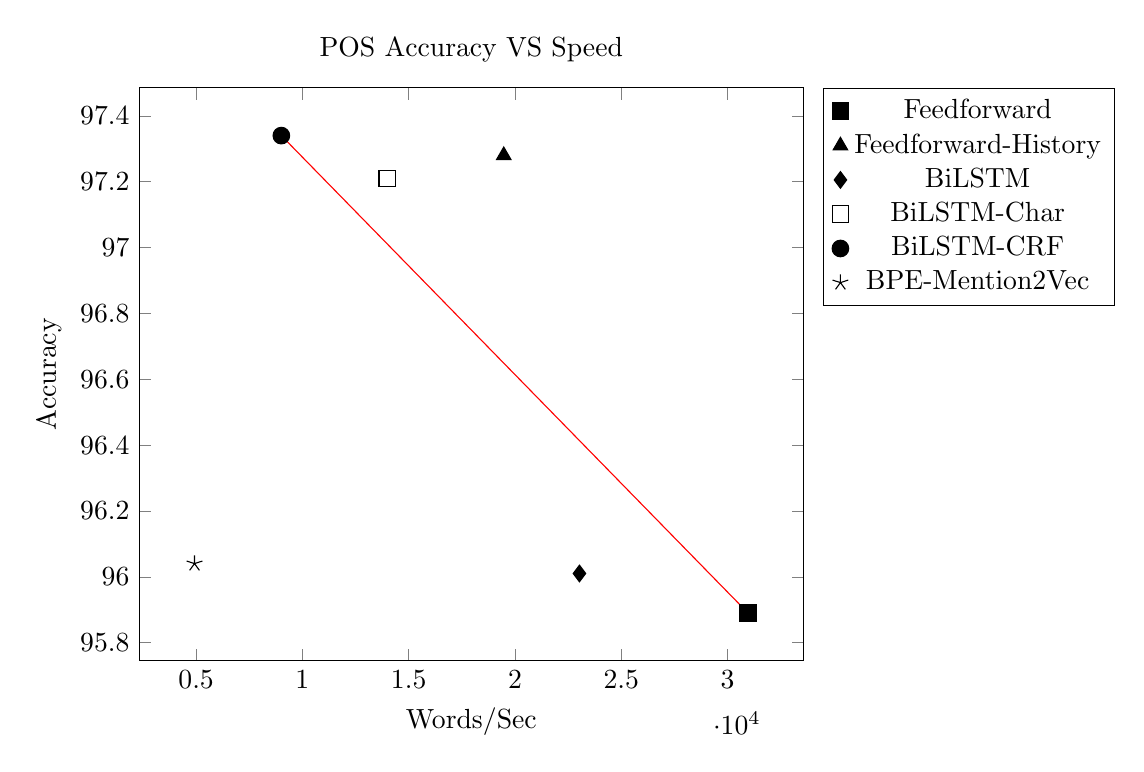
\begin{tikzpicture}
	\begin{axis}[%
	ylabel={Accuracy},
	xlabel={Words/Sec},
	scale only axis,
	mark size=3.0pt,
	title={POS Accuracy VS Speed},
	scatter/classes={%
		Feedforward={mark=square*},%
		Feedforward-History={mark=triangle*},%
		BiLSTM={mark=diamond*},%
		BiLSTM-Char={mark=square},
		BiLSTM-CRF={mark=otimes*},%
		BPE-Mention2Vec={mark=star}},%
	legend style={at={(1.03,1)},anchor=north west,draw=black,fill=white,align=left}]
	\addplot[scatter,only marks,%
		scatter src=explicit symbolic]%
	table[meta=label] {
    x     y      label
    30967  95.89  Feedforward 
    19474  97.28  Feedforward-History 
    23036  96.01  BiLSTM
    13992  97.21  BiLSTM-Char
    9009   97.34  BiLSTM-CRF
    4923   96.04  BPE-Mention2Vec
    };
    \addplot+ [mark=none]table {
    x     y      label
    30967   95.89   Feedforward  
    9009   97.34    BiLSTM-CRF
    };
	\addlegendentry{Feedforward}
	\addlegendentry{Feedforward-History}
	\addlegendentry{BiLSTM}
	\addlegendentry{BiLSTM-Char}
	\addlegendentry{BiLSTM-CRF}
	\addlegendentry{BPE-Mention2Vec}
	\end{axis}
\end{tikzpicture}
 \caption{Results of the POS system using different Neural Network Models}
  \label{fig:pos}
\end{figure}

Figure \ref{fig:ner} illustrates the trade-off between performance and speed of using different neural network models on CoNLL 2003. BiLSTM--CRF achieves the highest F1 Score 90.05, and Mention2Vec obtains the second best F1 Score 89.06. Feedforward achieves the fastest decoding speed since it employs a simple neural network with no extra features. The line in Figure \ref{fig:ner} connects the BiLSTM-CRF model which is the most accurate model and the Feedforward model which is the fastest model. The models above the line are faster but perform slightly worse than BiLSTM-CRF, such as Feedforward-History. Models below the line are slower and less accurate, which makes them less ideal for NER. Our new model, Feedforward-Mention2Vec, comes very close to the line, and it achieves 88.6 F1 score which is close to the best performance, and it is 1.3 times faster than the fully structured BiLSTM model.

\begin{figure}
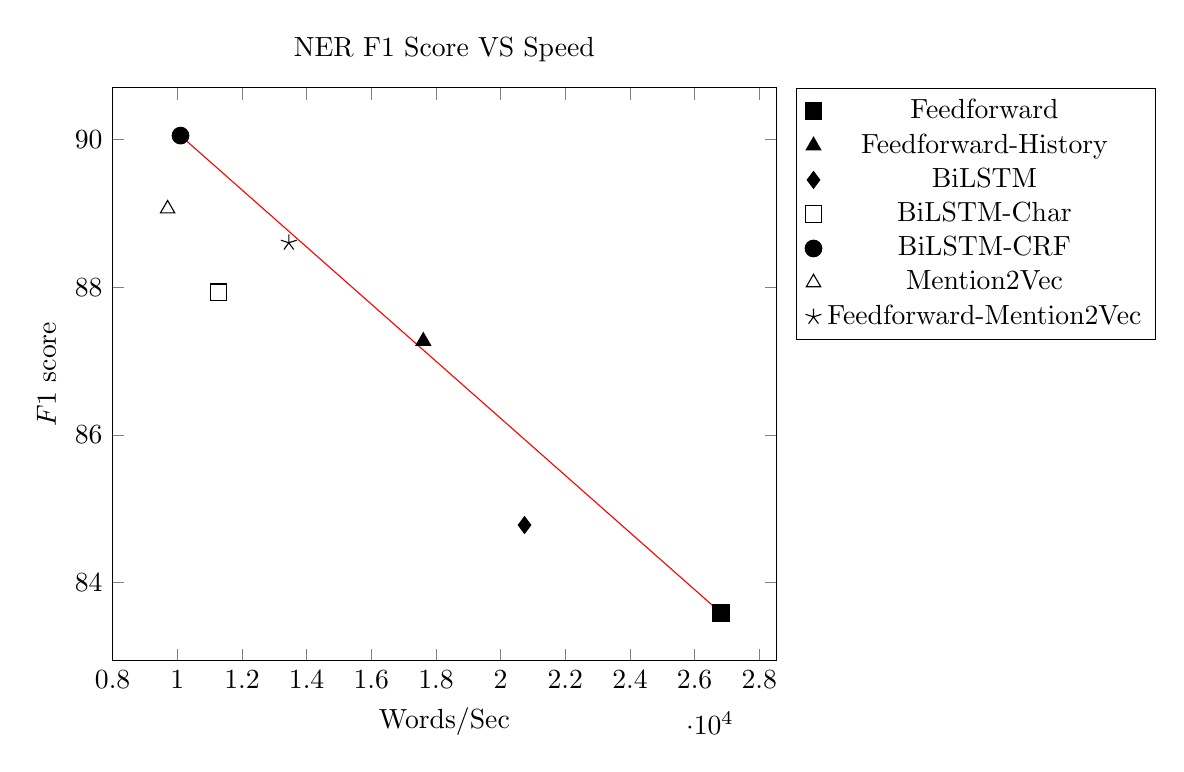
\begin{tikzpicture}
	\begin{axis}[%
	ylabel={$F1$ score},
	xlabel={Words/Sec},
	scale only axis,
	mark size=3.0pt,
	title={NER F1 Score VS Speed},
	scatter/classes={%
		Feedforward={mark=square*},%
		Feedforward-History={mark=triangle*},%
		BiLSTM={mark=diamond*},%
		BiLSTM-Char={mark=square},
		BiLSTM-CRF={mark=otimes*},%
		Mention2Vec={mark=triangle},
		Feedforward-Mention2Vec={mark=star}},%
	legend style={at={(1.03,1)},anchor=north west,draw=black,fill=white,align=left}]
	\addplot[scatter,only marks,%
		scatter src=explicit symbolic]%
	table[meta=label] {
    x     y      label
    26819   83.59   Feedforward 
    17609   87.27   Feedforward-History 
    20740   84.78   BiLSTM 
    11271   87.93   BiLSTM-Char
    10100   90.05   BiLSTM-CRF
    9701    89.06   Mention2Vec
    13450   88.6   Feedforward-Mention2Vec
	};
	\addplot+ [mark=none]table {
    x     y      label
    26819   83.59    Feedforward 
    10100   90.05   BiLSTM-CRF
    };
	\addlegendentry{Feedforward}
	\addlegendentry{Feedforward-History}
	\addlegendentry{BiLSTM}
	\addlegendentry{BiLSTM-Char}
	\addlegendentry{BiLSTM-CRF}
	\addlegendentry{Mention2Vec}
	\addlegendentry{Feedforward-Mention2Vec}
	\end{axis}
\end{tikzpicture}
 \caption{Results of the NER system using different Neural Network Models on CoNLL 2003}
  \label{fig:ner}
\end{figure}

Figure \ref{fig:chunking} illustrates the trade-off between performance and speed of using different neural network models on CoNLL 2000. BiLSTM-CRF achieves the highest F1 Score 93.86, and Mention2Vec obtains the second best F1 Score 89.06. Feedforward achieves the fastest decoding speed since it employs a simple neural network with no extra features. The line in Figure \ref{fig:ner} connects the BiLSTM-CRF model which is the most accurate model and the Feedforward model which is the fastest model. The models above the line are faster but perform slightly worse than BiLSTM-CRF, such as Feedforward-History. Models below the line are slower and less accurate, which makes them less ideal for Chunking.


\begin{figure}
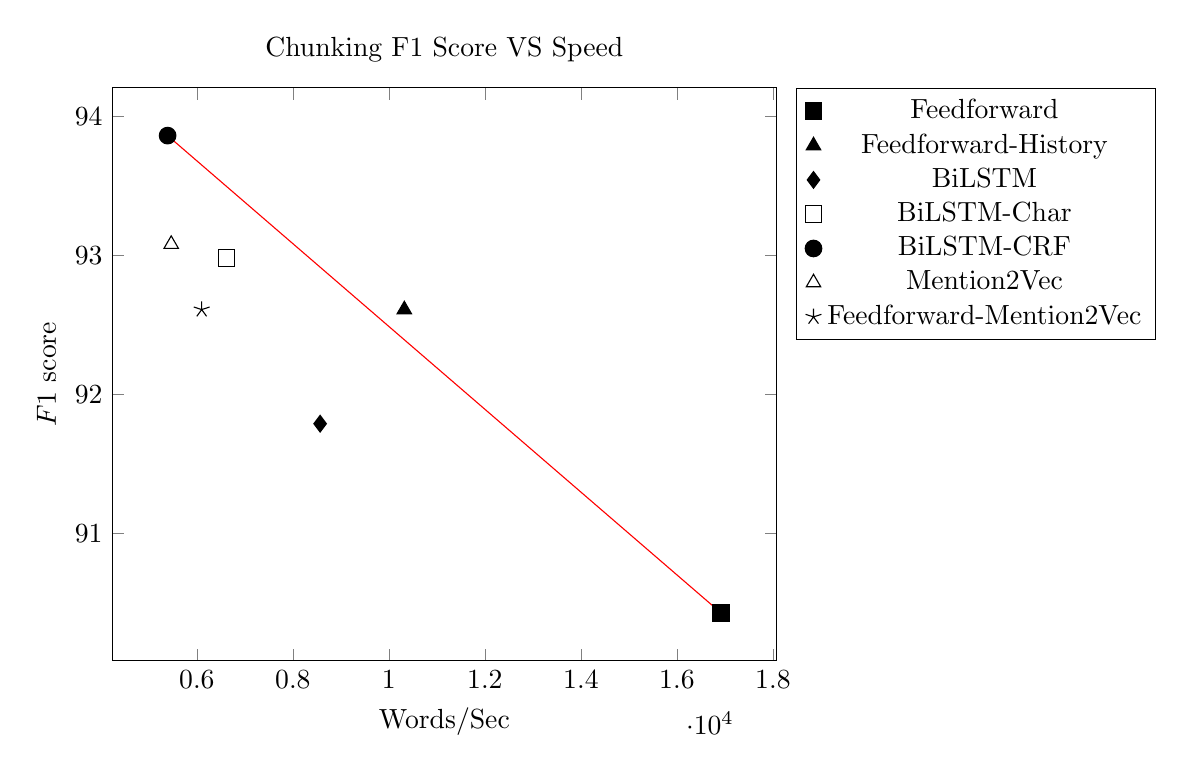
\begin{tikzpicture}
	\begin{axis}[%
	ylabel={$F1$ score},
	xlabel={Words/Sec},
	scale only axis,
	mark size=3.0pt,
	title={Chunking F1 Score VS Speed},
	scatter/classes={%
		Feedforward={mark=square*},%
		Feedforward-History={mark=triangle*},%
		BiLSTM={mark=diamond*},%
		BiLSTM-Char={mark=square},
		BiLSTM-CRF={mark=otimes*},%
		Mention2Vec={mark=triangle},
		Feedforward-Mention2Vec={mark=star}},%
	legend style={at={(1.03,1)},anchor=north west,draw=black,fill=white,align=left}]
	\addplot[scatter,only marks,%
		scatter src=explicit symbolic]%
	table[meta=label] {
    x     y      label
    16920   90.43   Feedforward 
    10321   92.61   Feedforward-History 
    8567    91.79   BiLSTM 
    6616    92.98   BiLSTM-Char
    5390    93.86   BiLSTM-CRF
    5465    93.08   Mention2Vec
    6100    92.61   Feedforward-Mention2Vec
	};
	\addplot+ [mark=none]table {
    x     y      label
   16920   90.43    Feedforward 
   5390    93.86   BiLSTM-CRF
    };
	\addlegendentry{Feedforward}
	\addlegendentry{Feedforward-History}
	\addlegendentry{BiLSTM}
	\addlegendentry{BiLSTM-Char}
	\addlegendentry{BiLSTM-CRF}
	\addlegendentry{Mention2Vec}
	\addlegendentry{Feedforward-Mention2Vec}
	\end{axis}
\end{tikzpicture}
 \caption{Results of the Chunking system using different Neural Network Models on CoNLL 2000}
  \label{fig:chunking}
\end{figure}

As illustrated in Figure \ref{fig:pos}, Figure \ref{fig:ner} and Figure \ref{fig:chunking}, the greedy sequence tagging systems using a feedforward network (Feedforward-History) can achieve comparable performance and faster speed than the systems using recurrent models; the multitask model (Feedforward-Mention2Vec) performs competitively with the state-of-the-art model on NER.

\begin{table}[]
\centering
\caption{F1 Scores and Decoding Speed on CoNLL 2003 and OntoNotes }
\label{table:my-label3}
\begin{tabular}{|c|c|c|c|c|}
\hline
& \multicolumn{2}{c|}{F1 Score} & \multicolumn{2}{c|}{Decoding Speed (Words/Sec)} \\ \hline
& CoNLL 2003     & OntoNotes    & CoNLL 2003              & OntoNotes             \\ \hline
Feedforward-Mention2Vec & 88.6          & 82.57        & 13445 (1.3$\times$)                  & 10812 (1.4$\times$)               \\ \hline
BiLSTM-CRF         & 90.05          & 85.90        & 10100                   & 7667                  \\ \hline
\end{tabular}
\end{table}

Table \ref{table:my-label3} compares the performance and decoding speed of BiLSTM-CRF and Feedforward-Mention2Vec on CoNLL 2003 and OntoNotes. It shows that Feedforward-Mention2Vec with a simple architecture can achieve competitive performance with BiLSTM-CRF on CoNLL 2003 and OntoNotes. The speed gap between Feedforward-Mention2Vec and BiLSTM-CRF grows as the number of named entity type increases. There is more speed benefit in using a multitask model like Feedforward-Mention2Vec when there are more named entity types to classify. 



